% Chapter 6

\chapter{Results} % Main chapter title
\section{Charged Track $v_{2}$}
\label{sect:alltracks}
%Add background contamination discussion, 3 point tracking vs 5 point tracking
Here I present measurements of elliptic flow in $\sqrt{s_{NN}}=200$ GeV d+Au collisions. Recall that the Fourier coefficients parameterize the shape of the azimuthal hydrodynamic flow by describing it as a superposition of cosine harmonics:
\begin{equation} \label{eq:frrexpanded}
\frac{d^{2}N}{dp^{2}} \propto v_0 + v_1 \cos\big(\phi - \Psi^{RP}_1\big) + v_2 \cos\big(2(\phi - \Psi^{RP}_2)\big) + v_3 \cos\big(3(\phi - \Psi^{RP}_3)\big) \cdots
\end{equation}
where $v_0$, $v_1$, $v_2$, and $v_3$ are the values that scale the amount of spherical, directed, elliptic, and triangular flow respectively, and are indicative of collective behavior of the nuclear matter. The angle, $\phi$, is the azimuthal angle in the lab frame and $\Psi^{RP}_n$ is the angle of the reaction plane in the lab frame\footnote{for the $n$-th Fourier harmonic.}. This can be simplified by defining the coordinate: $\Delta \phi = \phi - \Psi^{RP}_n$ which gives:
\begin{equation} 
\frac{d^{2}N}{dp^{2}} \propto v_0 + v_1 \cos(\Delta \phi _1) + v_2 \cos(2\Delta \phi _2) + v_3 \cos(3\Delta \phi _3) \cdots
\end{equation}
effectively redefining eqn. \ref{eq:frrexpanded} relative to the event plane. To measure the elliptic flow ($v_2$) we count number of tracks in bins of $\Delta \phi_2$ and fit this with a function of the form:
\begin{equation}
\label{v2fitfn}
f(\Delta \phi_2) = v_0 [1 + v_2 \cos 2 \Delta \phi_2]
\end{equation}
where $v_0$ is a term that accounts for an overall shift in the number of tracks due to statistics and $v_2$ is the 2nd order Fourier harmonic of the azimuthal momentum anisotropy. By the orthogonality of Fourier harmonics and because the event plane is determined for each harmonic independently\footnote{and therefore $\Delta \phi$ is specific to a particular harmonic.}, all other $v_n$ contributions must be calculated independently.


\section{Separating Particle Signals}
Following the recentering of the Q vectors, the flattening of the event plane, and checking for calibration of the TOF detector, 2-d histograms of $p_T$ vs $m^2$ are plotted following the method described in section \ref{sect:pidmethod} to identify the species of charged track hits in the TOF. 
\begin{figure}[htbp!]
  \centering
    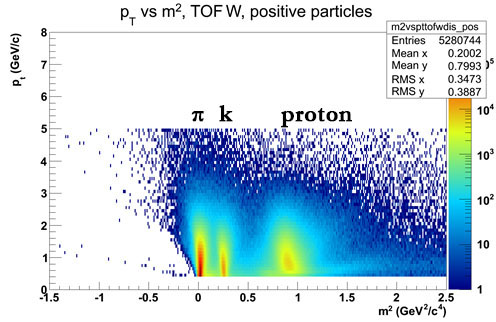
\includegraphics[width=1\textwidth]{Figures/ptvsm2tof.jpg}
    \rule{35em}{0.5pt}
  \caption[Track $p_T$ vs $m^2$ determined by the TOF.W showing separation of $\pi$, k, and proton particle signals.]{Track $p_T$ vs $m^2$ determined by the TOF.W showing separation of $\pi$, k, and proton particle signals.}
  \label{fig:accspread}
\end{figure}

In order to do a statistical analysis, these 2-d histograms will need to be ``sliced'' into a series of 1-d histograms in small bins of $p_T$ which will give a 3-peak histogram showing the signatures of the pion, kaon, and proton which are Gaussian in shape. There are 15 bins of $p_T$ starting at $0.5 \leq p_T \leq 0.7$ GeV/c and increasing by steps of 0.2 GeV/c per bin up to $p_T = 2.9$. At this point, to increase statistics, bins are increased to 0.5 GeV/c per increment for the last 3 bins, starting at $p_T = 3.0$ GeV/c, up to $p_T = 4.5 $ GeV/c. Over the range of $p_T$ in this analysis, the widths and heights of the particle peaks will change and overlap in various ways, because of this I will divide the $p_T$ range into three ranges, each of which will be analyzed with different methods with corresponding systematics. After fitting the particle distributions, the Gaussian fit functions are then integrated to calculate the particle yield for each species. Integration bounds can be set to increase track ID purity at the expense of statistics and vice versa. The yields from the integrated Gaussians of each particle species are then fit with the Fourier function to determine the 2nd harmonic coefficient as per equation \ref{v2fitfn}. 

\subsection{Single Gaussians}
\begin{figure}[htbp!]
  \centering
    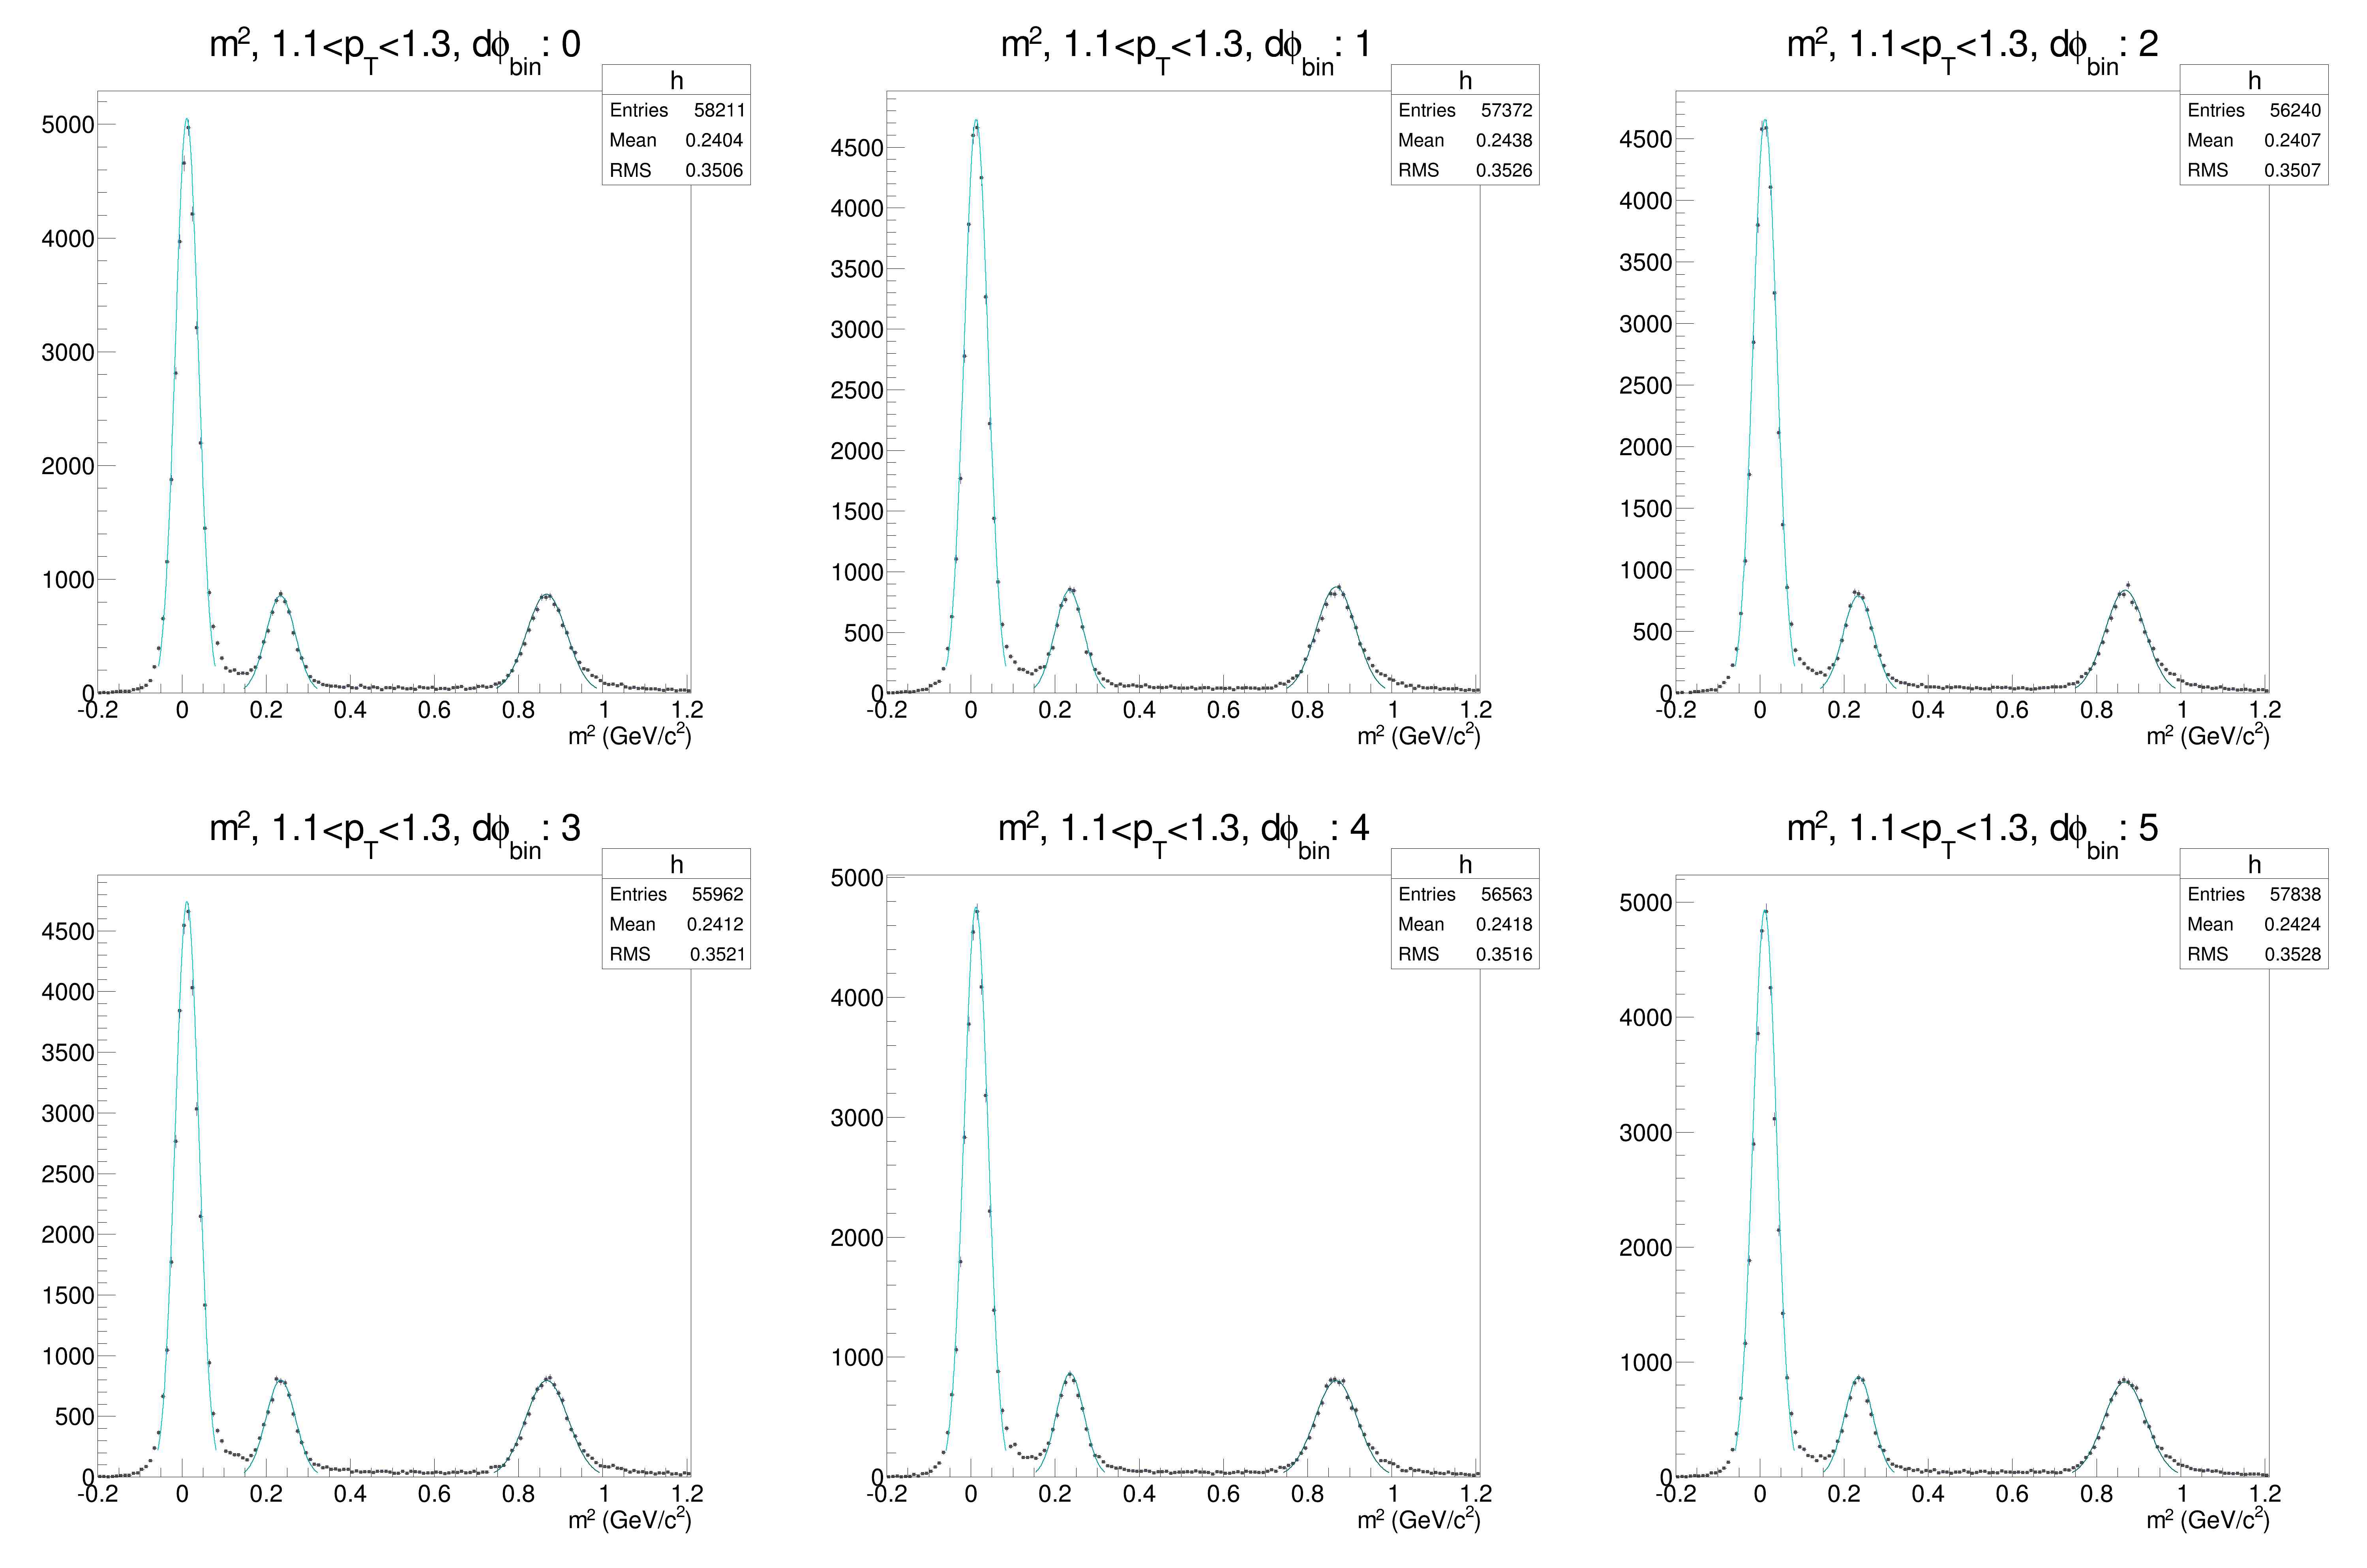
\includegraphics[width=0.8\textwidth]{lowptfits/yieldvsdphi_tof1_cent0_ch1_pT-11-13.jpg}
    \rule{35em}{0.5pt}
  \caption[Example single Gaussian fits of $m^2$ for $p_T\leq1.3$ GeV/c in 6 bins of $\Delta \phi$.]{Example single Gaussian fits of $m^2$ for $p_T\leq1.3$ GeV/c in 6 bins of $\Delta \phi$.}
  \label{fig:singlegausm2}
\end{figure}

For $p_T< 1.3$, there is enough separation between the pion, kaon, and proton signals to fit each particle peak with a single Gaussian (fig. \ref{fig:singlegausm2}). This will take the form:
\begin{equation}
f(m^2) = \frac{N_0}{\sqrt{2\pi \sigma^2}} e^{-\frac{(m^2-\mu)^2}{2\sigma^{2}}},
\end{equation}
where $\sigma$ is the width of the identified particle peak, $\mu$ is the location of the peak's mean along the x-axis, and $N_0$ is the height of the peak. To determine the identified particle yield, the Gaussians are then integrated from $\mu-2\sigma$ to $\mu+2\sigma$ for each particle distribution, i.e. the number of particles of each type are counted out to two standard deviations around their mean mass. Since the means of the mass and the widths of the mass distributions are not expected to change in bins of $\Delta \phi$, as a check, the values of the means and the widths are plotted for the specific bin of $p_T$ in order to verify that they do not change. The yields for each particle species are also plotted in the bins of $\Delta \phi$ (fig. \ref{fig:yieldphisinglegaus}). (full set of fits and data can be seen in Appendix \ref{app:singlegauss})

\begin{figure}[htbp!]
  \centering
    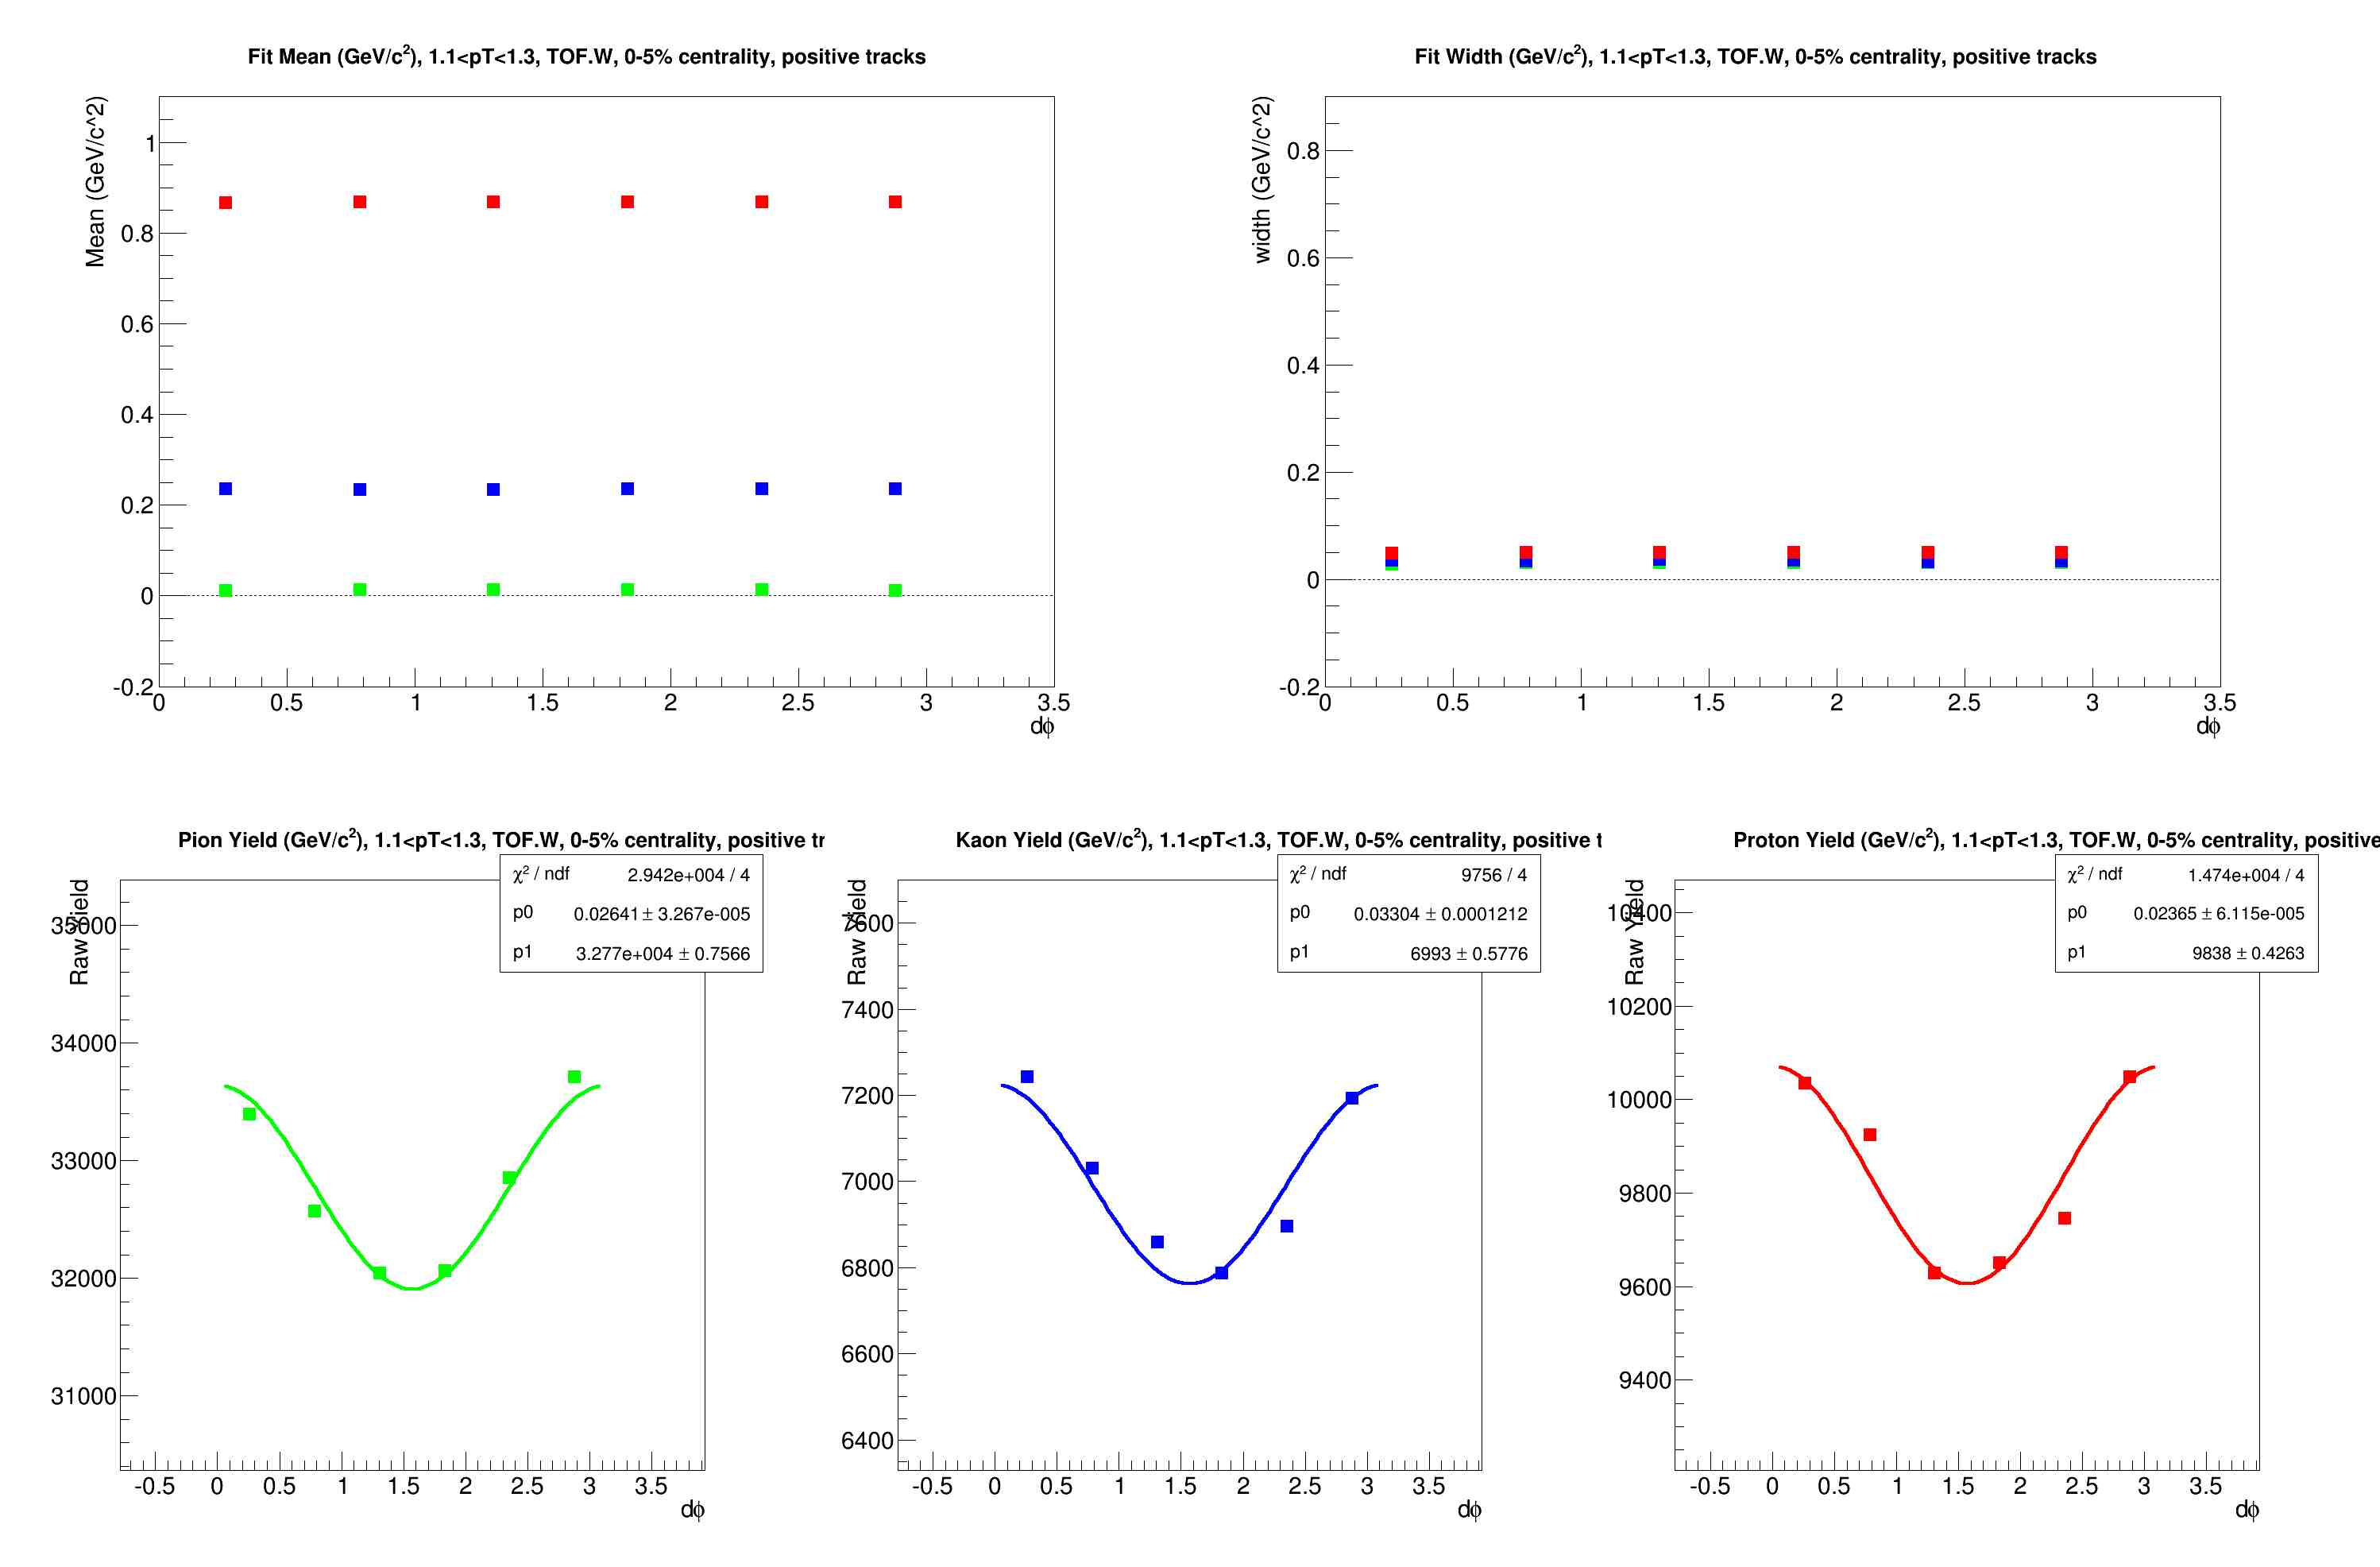
\includegraphics[width=0.8\textwidth]{lowptfits/fitParams_tof1_cent0_ch1_pT-11-13.jpg}
    \rule{35em}{0.5pt}
  \caption[Particle distribution fit mean and width QA. $\pi$, k, p yield vs $\Delta \phi$ and corresponding Fourier fits for $p_T\leq 1.3$ GeV/c.]{Particle distribution fit mean and width QA, $\pi$, k, p yield vs $\Delta \phi$ and corresponding Fourier fits for $p_T\leq 1.3$ GeV/c.}
  \label{fig:yieldphisinglegaus}
\end{figure}

\subsection{Multiple Gaussians}
\begin{figure}[htbp!]
  \centering
    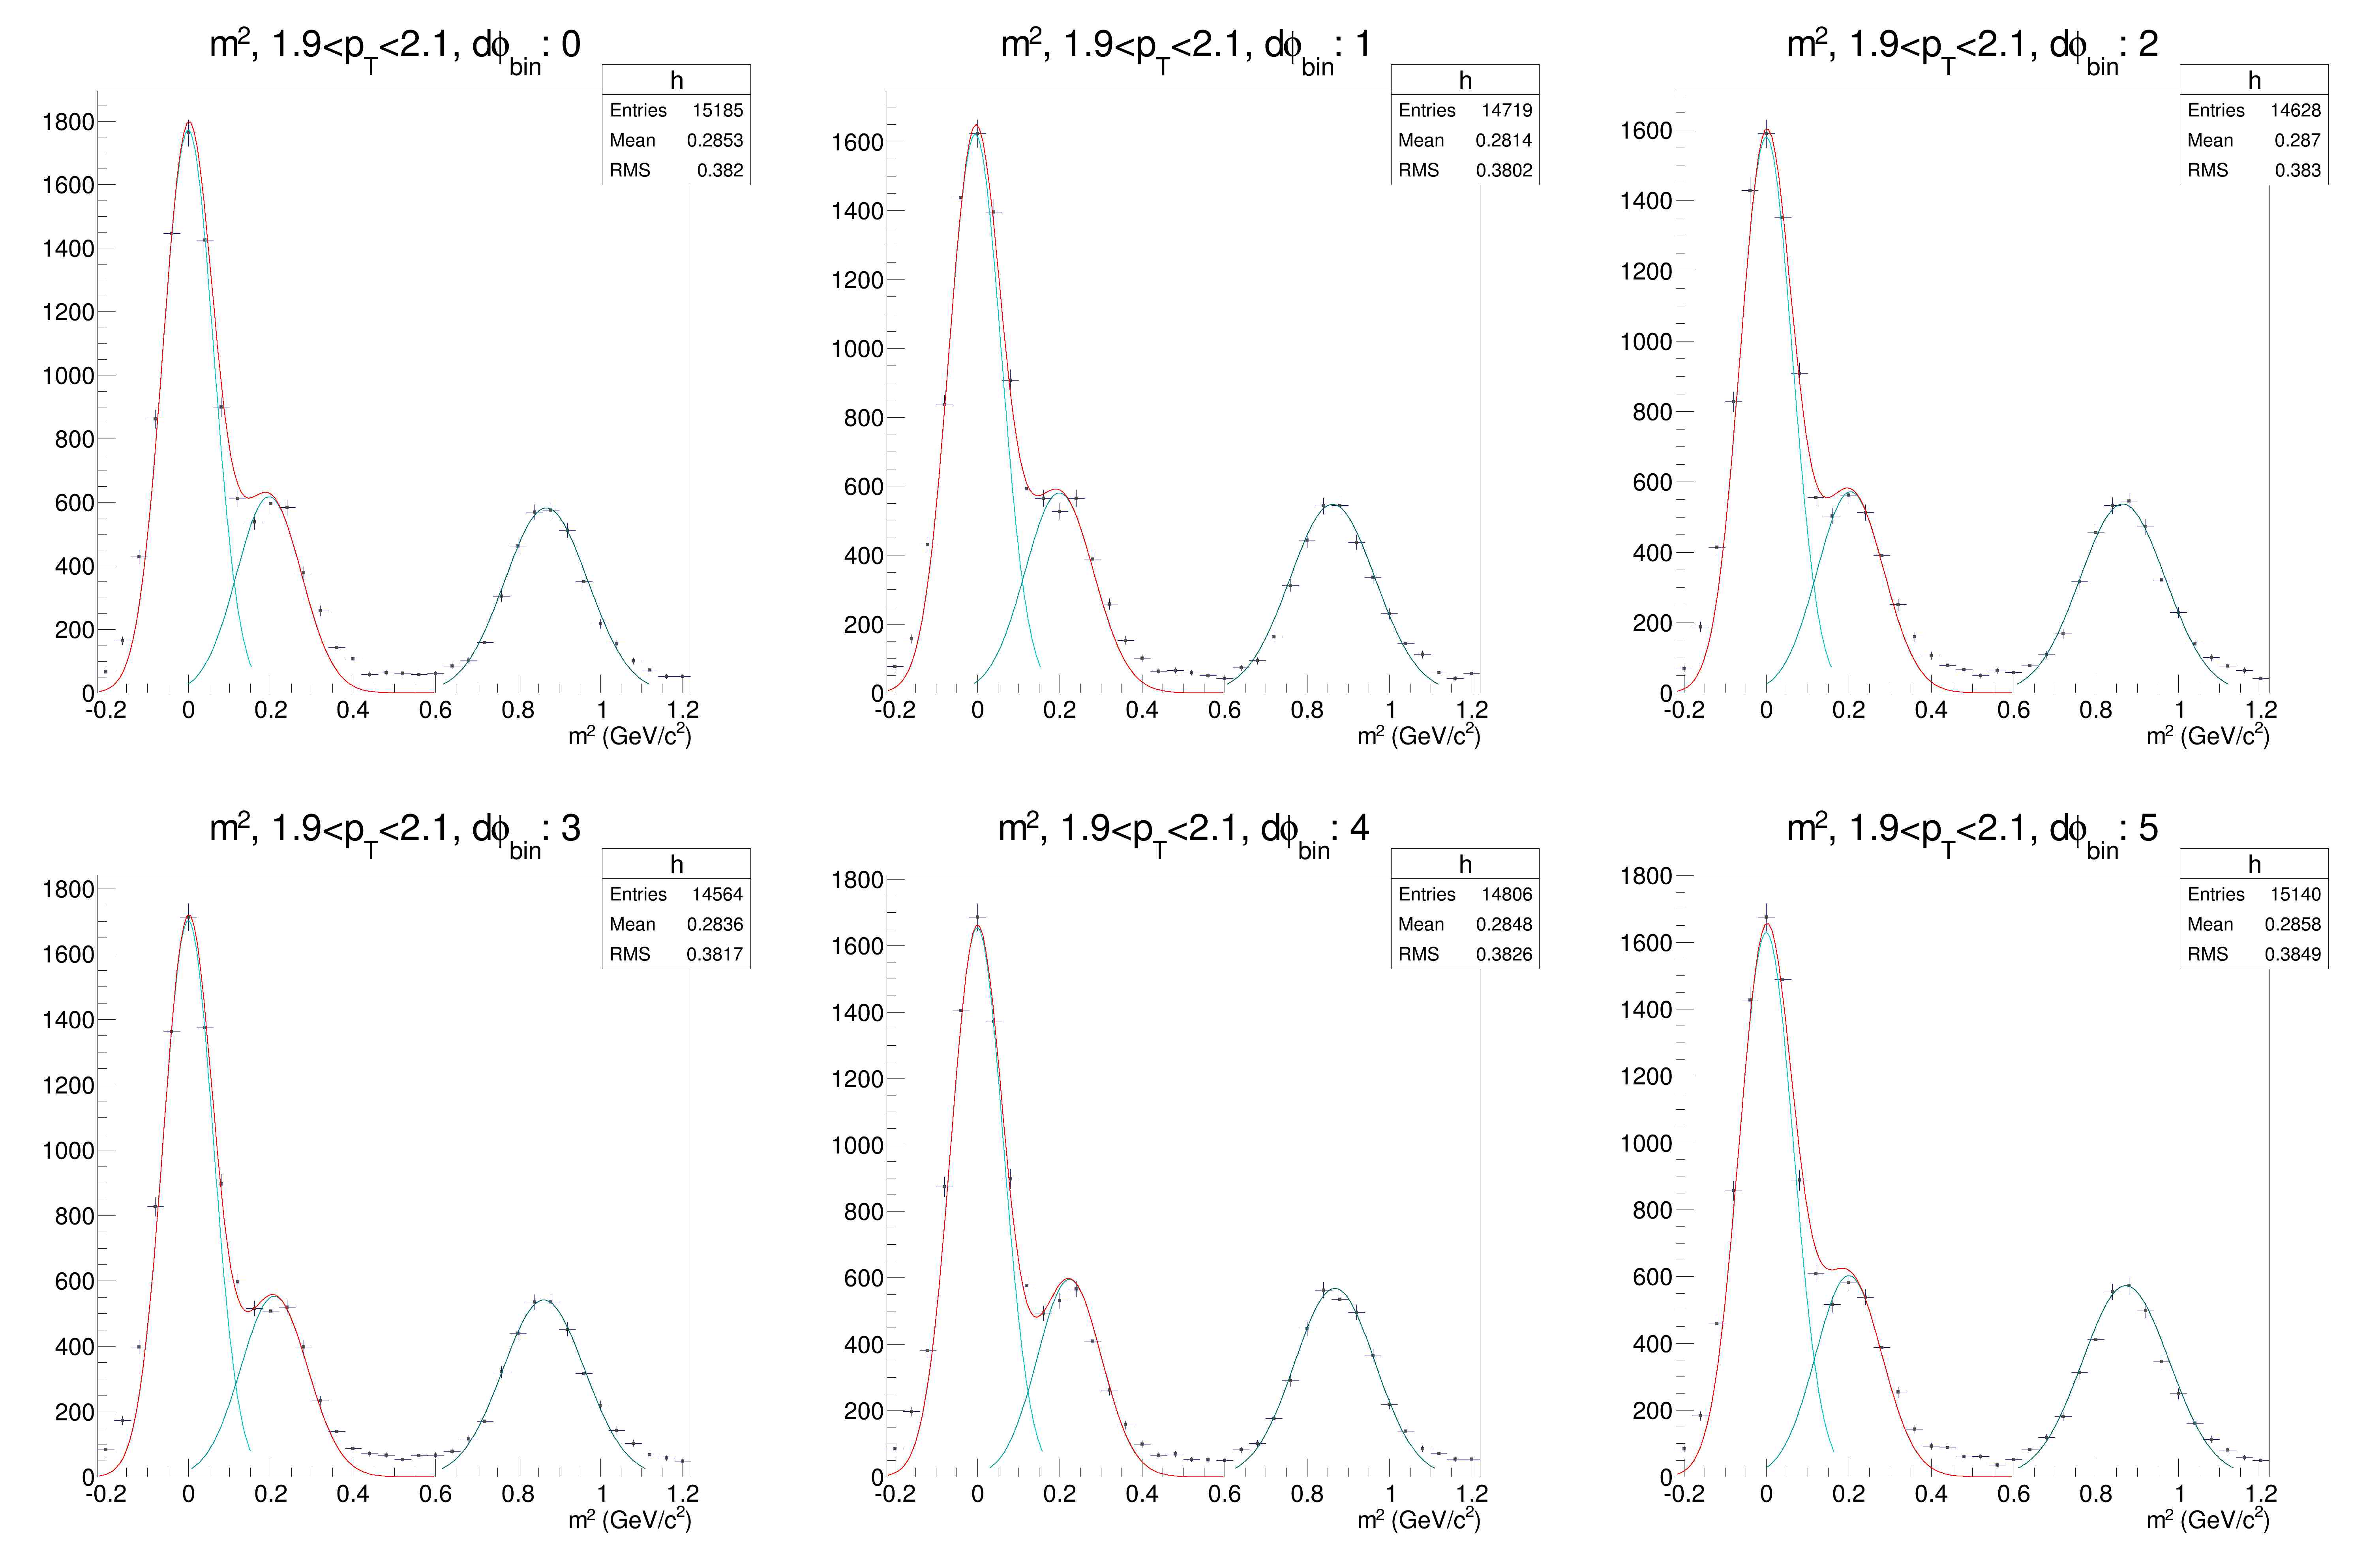
\includegraphics[width=0.8\textwidth]{lowptfits/yieldvsdphi_tof1_cent0_ch1_pT-19-21.jpg}
    \rule{35em}{0.5pt}
  \caption[Example mixed Gaussian fits of $m^2$ for $1.3 \leq p_T\leq 2.1$ GeV/c in 6 bins of $\Delta \phi$.]{Example mixed Gaussian fits of $m^2$ for $1.3 \leq p_T\leq 2.1$ GeV/c in 6 bins of $\Delta \phi$.}
  \label{fig:mixgausm2}
\end{figure}
For $1.3<p_T<2.1$, kaon and pion mass distributions become overlapped. To decouple the two I fit the distribution with a combination of two Gaussians in order to fit the overlapping tails of the distributions without over counting (see fig. \ref{fig:mixgausm2}). This function takes the form:
\begin{equation}
f(m^2) = \frac{1}{\sqrt{2\pi}} \bigg( \frac{N_{\pi}}{\sigma_{\pi}} e^{-\frac{(m^2-\mu_{\pi})^2}{2\sigma_{\pi}^{2}}} + \frac{N_{k}}{\sigma_{\pi}-\sigma_{k}} e^{-\frac{(m^2-\mu_{k})^2}{2(\sigma_{\pi} - \sigma_{k})^{2}}} \bigg),
\end{equation}
where $N_{x}$, $\mu_x$, and $\sigma_x$ are the parameters that describe the shape of particle $x$'s ($\pi$/k) distribution. These parameters can then be used to reconstruct single Gaussian distributions which are then integrated out to $2\sigma$ as mentioned in the previous section.
(full fits and data in Appendix \ref{app:mixgauss}).

Triple Gaussian fits were attempted, however pion and kaon peaks were so strongly merged that many possible ratios of pion and kaon heights reproduced the same peak in the data. This occurs in a region where the ACC can be utilized so a triple Gaussian fit attempt was abandoned.

\subsection{ACC as a Particle Discriminator}

\begin{sidewaysfigure}[p]
  \centering
    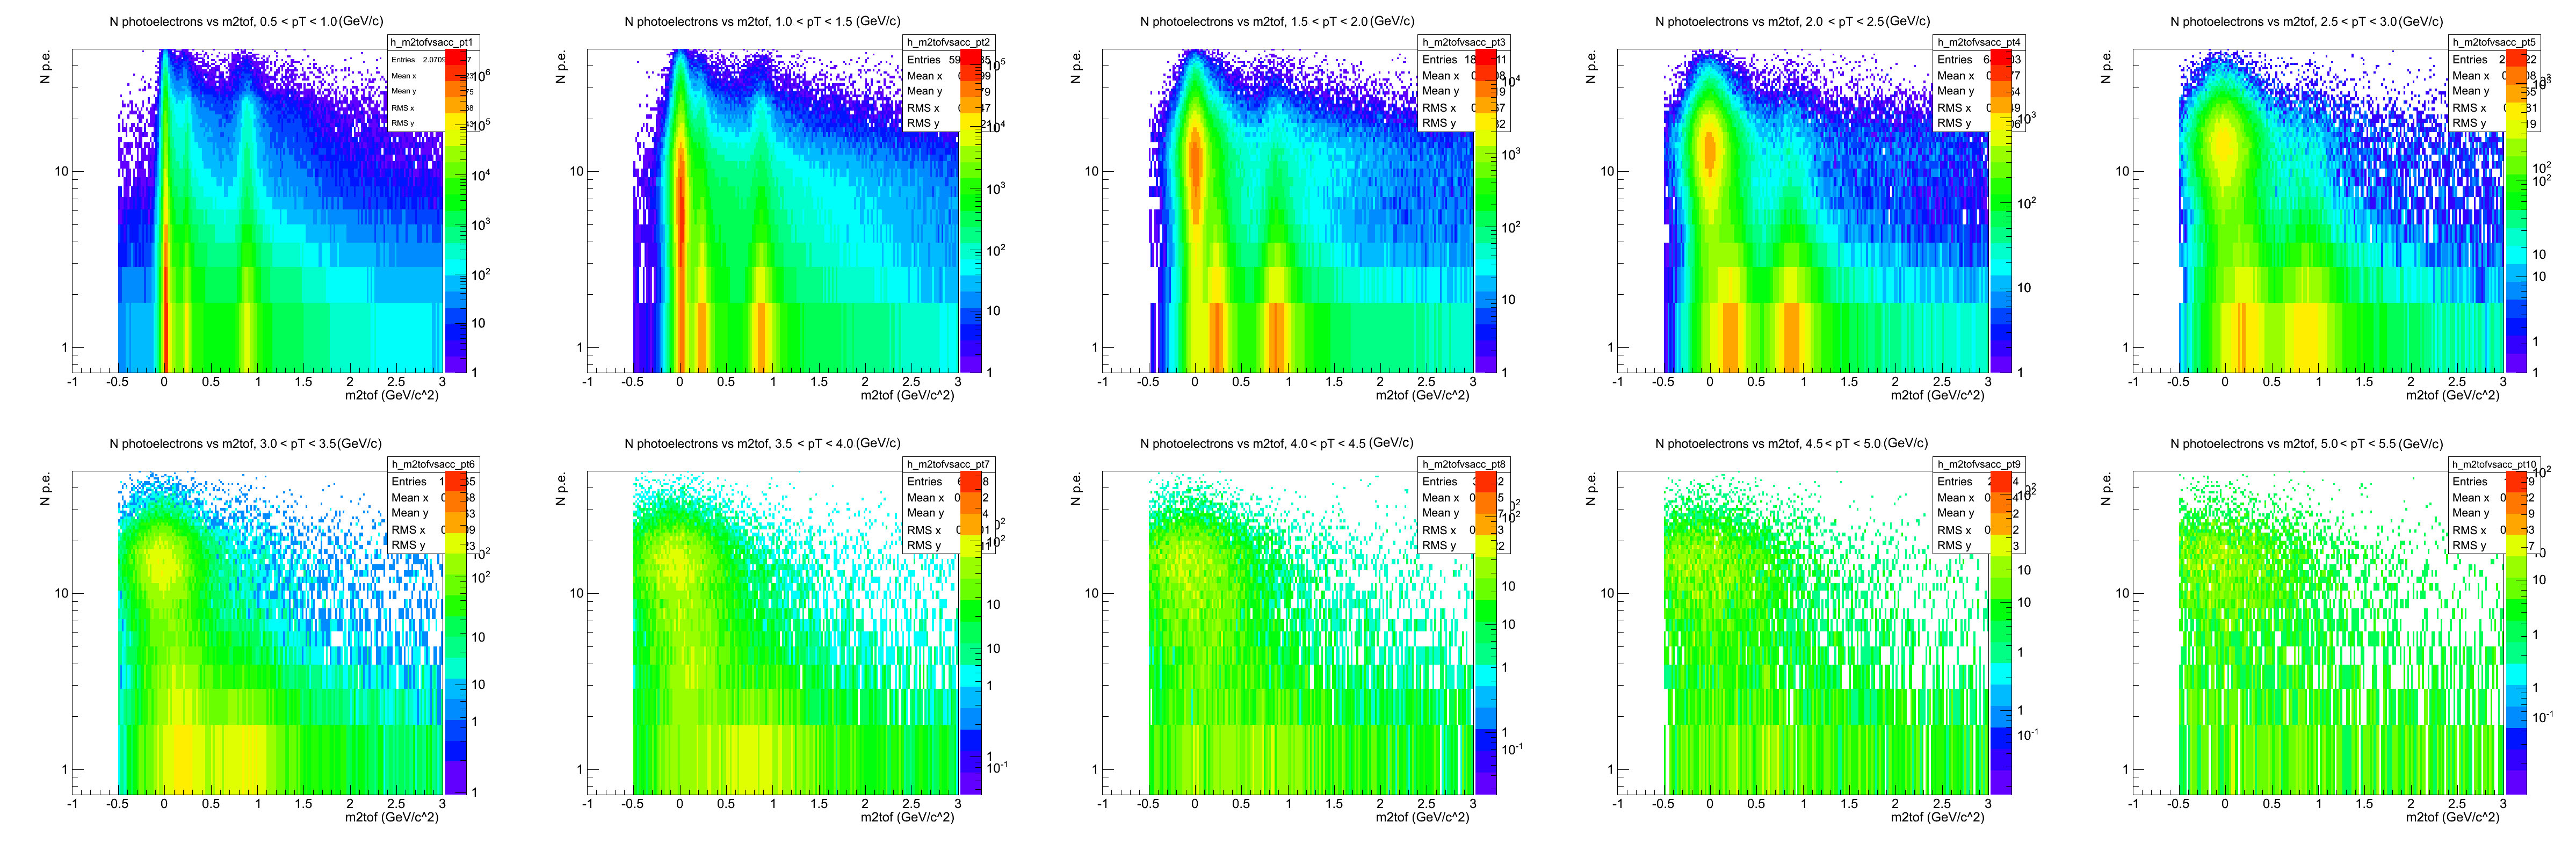
\includegraphics[width=1.1\textwidth]{hiptfits/nphotvsm2.jpg}
    \rule{35em}{0.5pt}
  \caption[Number of ACC photoelectrons vs $m^2$ in bins of $p_T$.]{Number of ACC photoelectrons vs $m^2$ in bins of $p_T$. As $p_T$ increases, the number of ACC photoelectrons can be used to discriminate pions from kaons and protons.}
  \label{fig:accspread}
\end{sidewaysfigure}

Above $p_T=2.3$ pion/kaon mixing becomes inseparable. In this region I utilize the ACC to trigger and veto pion and kaon events respectively by setting Cherenkov radiation threshold which is done by counting the number of photoelectrons collected by the two PMTs on each channel of the ACC (see fig. \ref{fig:accspread}). This utilization of the ACC therefore sorts tracks into two separate histograms, one with an \textit{ACC fire} condition that contains mostly pions with minimal kaon contamination, and another with an \textit{ACC veto} condition that contains the remaining kaons and protons with minimal pion contamination. These two histograms can then be analyzed with single Gaussians since the distributions are now separate. This ACC threshold is the sum of the number of photoelectrons ($N_{p.e.}$) in both PMTs. The total number of $N_{p.e.}$ is plotted versus $m^2$ in a 2-d histogram and a threshold is set in order for there to be a maximum separation between pion and kaon signals. This 2-d histogram is then projected from the threshold up to the highest $N_{p.e.}$ bin for the pions and projected from the threshold down to the lowest $N_{p.e.}$ bin for kaons and protons. These 1-d projections can then be modeled with either single Gaussians (pions) or mixed Gaussians (kaons and protons). (full fits and data in Appendix \ref{app:accdata})

\subsection{High $p_T$: Fixed Width and Mean}
Above $p_T$=3.5, the strength of particle signatures decreases, approaching level of the background, making individual peaks hard to fit. Though statistics may be very low in the six bins of $d\phi$, there are still enough statistics if all the bins are combined. Means and widths of particle signals should only depend on $p_T$ and not on $d\phi$, therefore I can merge all $d\phi$ bins to calculate the statistical mean and width for each particle species at a given $p_T$ and fix these means and widths as constant for each bin in $d\phi$ and allow the heights of the Gaussians to dictate the yield.

\section{Identified Particle $v_{2}$}
The end result of each of these particle identification methods is a Yield vs $d\phi$ plot for the three particle species. These plots can be treated like the $dN/d\phi$ vs $d\phi$ plots that provided the charged track $v_2$ measurement which was acquired by fitting with the functional form of equation \ref{v2fitfn}. The parameters of this Fourier fit are the uncorrected $v_2$ coefficients. Dividing by the event plane resolution gives the corrected $v_2$ (fig \ref{fig:v2all}) (see section \ref{secteperr}). Statistical error bars on this plot come from the associated parameter errors in the Gaussian fits, propagated through and combined with the errors of the cosine fits. Systematic error bars are treated in the next chapter.

\begin{figure}[htbp!]
  \centering
    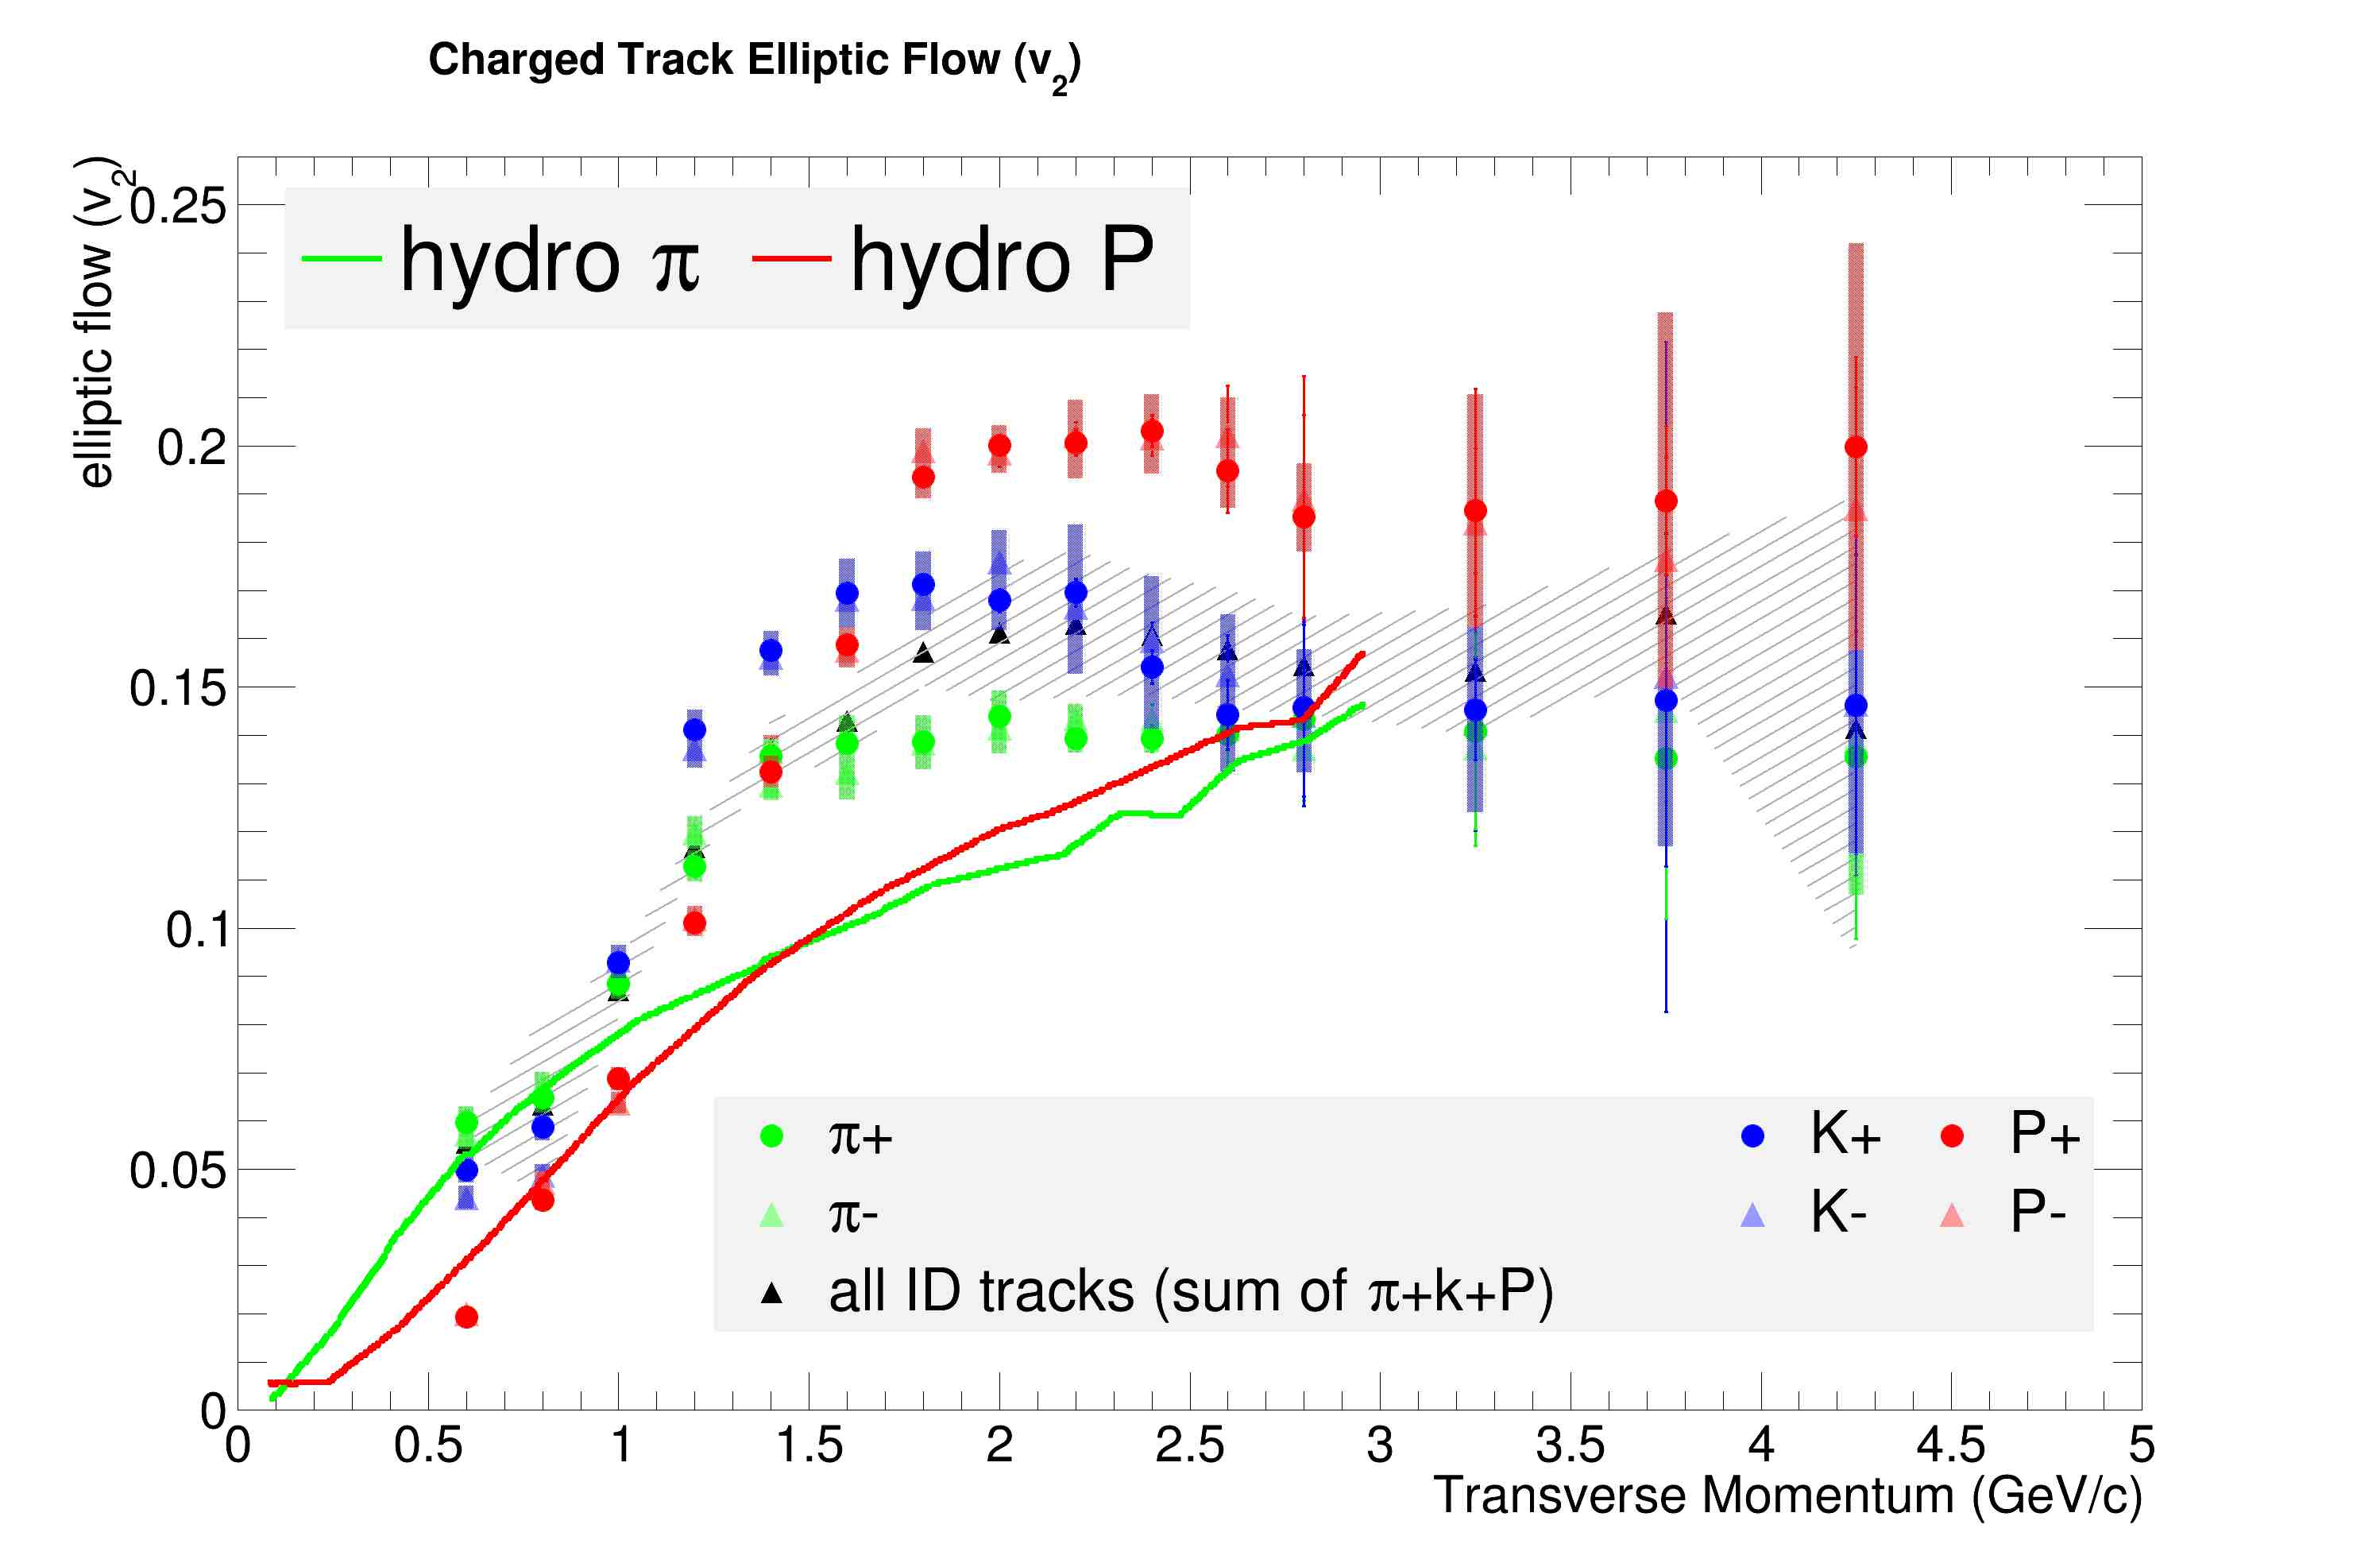
\includegraphics[width=1\textwidth]{v2all.jpg}
    \rule{35em}{0.5pt}
  \caption[$\pi^{\pm}$, $k^{\pm}$, $p/\bar{p}$ elliptic flow,$\sqrt{s_{NN}}=$200 GeV d+Au collisions]{$\pi^{\pm}$, $k^{\pm}$, $p/\bar{p}$ elliptic flow, resolution corrected.}
  \label{fig:v2all}
\end{figure}

\pagebreak
\pagebreak
